\section{Results}\label{sec:results}
Below are the results for the different test cases. The layout should be pretty
similar so they should be quite easy to follow.

To get some good results I ran all of the test cases several times testing the
different variables, these tests are not included here. One problem with this is
that I can't know for certain that this is good, because it can easily end up in
a local maximum regarding the different variables, e.g. I can test different
mutation rates, but find the best one when considered with all of the others.

\subsection{Test Case 1}\label{sec:test-case-1}
In this test we are testing STDM with the test case
\textit{izzy-train1.dat}.
\subsubsection{EA Parameters}\label{sec:test-case-1-parameters}
\begin{lstlisting}[frame=single, language=bash, caption=Command-line to
replicate the results]
python src/main.py 350 5 50 --mutation=0.1 --cross_rate=0.8 full_generational
tournament --k=5 --elite=3 stdm convert_neuron neuron_plot training\
data/izzy-train1.dat --bits_per_num=35 --e=0.02
\end{lstlisting}
\begin{table}[h]
	\begin{tabular}{c c}
		Variable & Value \\
		\hline
		Generations & 350 \\
		\hline
		Population size & 50 \\
		\hline
		Mutation rate & 0.1 \\
		\hline
		Crossover rate & 0.8 \\
		\hline
		Protocol & Full generational replacement \\
		\hline
		Mechanism & Tournament selection, k=5 and e=0.02 \\
		\hline
		Elitism & 3 \\
		\hline
		Bits per number & 35 \\
	\end{tabular}
	\caption{EA parameters for test case 1}
\end{table}
\subsubsection{End Results}\label{sec:test-case-1-results}
As we can see in figure \ref{fig:spike-test-case-1} the end result is quite good
for the STDM. Although for this test I had to up the bits per number to quite
high and had to run with a higher population than I had initially
wanted\footnote{Mostly do to performance concerns}. The end result is good and
there is nothing really special about this. From the last project I found that
\textit{Tournament selection} was the better of the four mechanisms and that is
reflected here, all the other did worse under the same conditions.

Looking at figure \ref{fig:fitness-test-case-1} we can see that the analysis
about the new crossover was quite right. If we look at the standard deviation we
can see that it is very low to begin with and then after some time, goes up. This
is signs of stagnation, but because of the high mutation rate we get a good end
result.
\begin{table}[h]
	\begin{tabular}{c c c c c}
		a & b & c & d & k \\
		\hline
		0.0323 & 0.0441 & -50.924 & 1.1294 & 0.0412
	\end{tabular}
	\caption{The neuron variables which gave the best solution for test case
	1}
\end{table}
\begin{figure}[h]
	\centering
	\begin{subfigure}[b]{0.5\textwidth}
		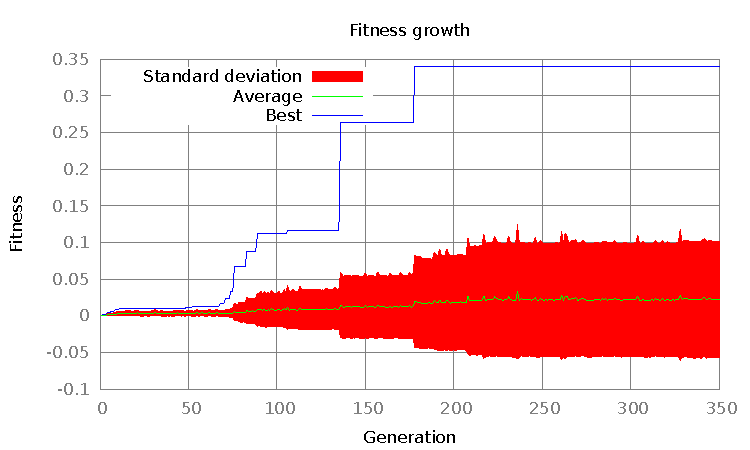
\includegraphics[width=\textwidth]{../output/stdm_izzy_1_fitness.pdf}
		\caption{Fitness progression for test case 1}
		\label{fig:fitness-test-case-1}
	\end{subfigure}%
	\begin{subfigure}[b]{0.5\textwidth}
		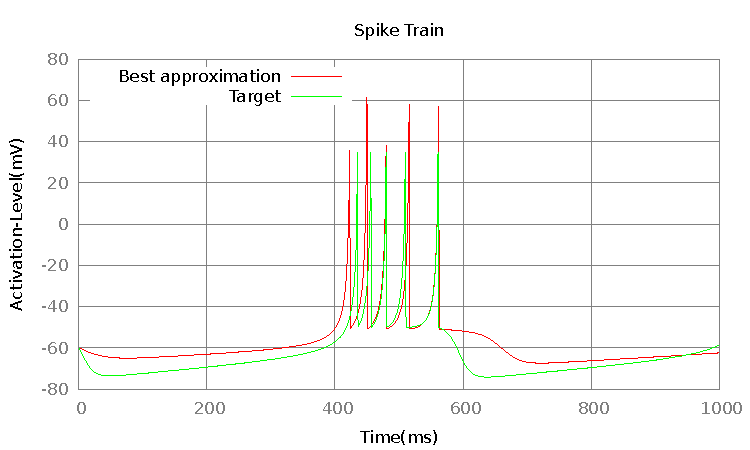
\includegraphics[width=\textwidth]{../output/stdm_izzy_1_spike.pdf}
		\caption{Spike train comparison for test case 1}
		\label{fig:spike-test-case-1}
	\end{subfigure}
	\caption{Test case 1 result}
\end{figure}

\subsection{Test Case 2}\label{sec:test-case-2}
In this test we are testing SIDM with the test case
\textit{izzy-train1.dat}.
\subsubsection{EA Parameters}\label{sec:test-case-2-parameters}
\begin{lstlisting}[frame=single, language=bash, caption=Command-line to
replicate the results]
python src/main.py 350 5 50 --mutation=0.05 --cross_rate=0.8 full_generational
tournament --k=5 --elite=3 sidm convert_neuron neuron_plot training\
data/izzy-train1.dat --bits_per_num=30 --e=0.02
\end{lstlisting}
\begin{table}
	\begin{tabular}{c c}
		Variable & Value \\
		\hline
		Generations & 350 \\
		\hline
		Population size & 50 \\
		\hline
		Mutation rate & 0.05 \\
		\hline
		Crossover rate & 0.8 \\
		\hline
		Protocol & Full generational replacement \\
		\hline
		Mechanism & Tournament selection, k=5, e=0.02 \\
		\hline
		Elitism & 3 \\
		\hline
		Bits per number & 30 \\
	\end{tabular}
	\caption{EA parameters for test case 2}
\end{table}
\subsubsection{End Results}\label{sec:test-case-2-results}
In figure \ref{fig:spike-test-case-2} we can see the spike train for this test
case, and the story is quite different from the last case, but it is quite
expected considering what SIDM actually does. Since it is mostly conserned with
the distance between spikes this technique is very good at getting the distance
right, but the placement in the spike train is often wrong.

The fitness(see figure \ref{fig:fitness-test-case-2}) for this case is much 
closer to the previous case than the spike
train. We can see that in the start the standard deviation is low, but then
after some, lucky, mutations it grows and we get a more diverse population.
\begin{table}
	\begin{tabular}{c c c c c}
		a & b & c & d & k \\
		\hline
		0.0010 & 0.0207 & -55.985 & 5.2820 & 0.0497
	\end{tabular}
	\caption{The neuron variables which gave the best solution for test case
	2}
\end{table}
\begin{figure}[h]
	\centering
	\begin{subfigure}[b]{0.5\textwidth}
		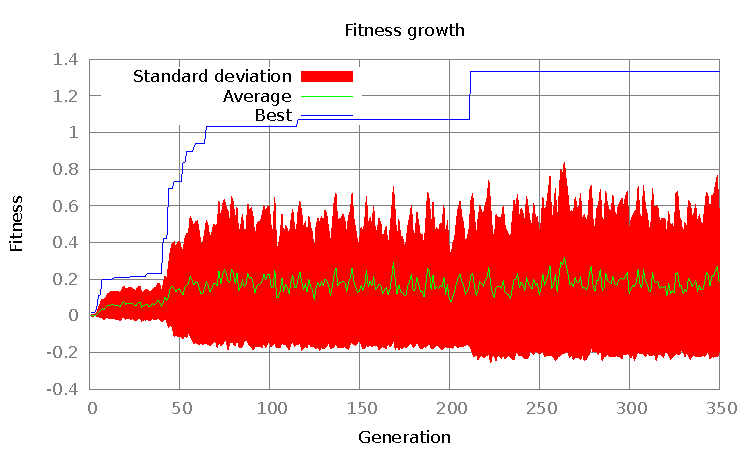
\includegraphics[width=\textwidth]{../output/sidm_izzy_1_fitness.pdf}
		\caption{Fitness progression for test case 2}
		\label{fig:fitness-test-case-2}
	\end{subfigure}%
	\begin{subfigure}[b]{0.5\textwidth}
		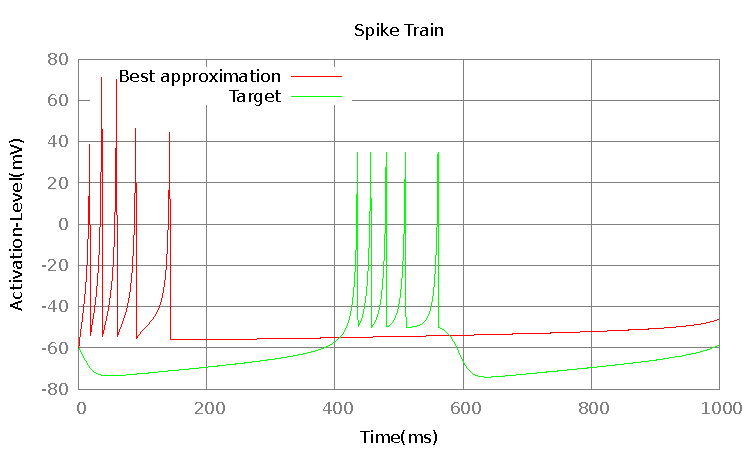
\includegraphics[width=\textwidth]{../output/sidm_izzy_1_spike.pdf}
		\caption{Spike train comparison for test case 2}
		\label{fig:spike-test-case-2}
	\end{subfigure}
	\caption{Test case 2 result}
\end{figure}

\subsection{Test Case 3}\label{sec:test-case-3}
In this test we are testing WDM with the test case
\textit{izzy-train1.dat}.
\subsubsection{EA Parameters}\label{sec:test-case-3-parameters}
\begin{lstlisting}[frame=single, language=bash, caption=Command-line to
replicate the results]
python src/main.py 500 5 50 --mutation=0.05 --cross_rate=0.7 full_generational
sigma --elite=3 wdm convert_neuron neuron_plot training\ data/izzy-train1.dat
--bits_per_num=20
\end{lstlisting}
\begin{table}
	\begin{tabular}{c c}
		Variable & Value \\
		\hline
		Generations & 500 \\
		\hline
		Population size & 50 \\
		\hline
		Mutation rate & 0.05 \\
		\hline
		Crossover rate & 0.7 \\
		\hline
		Protocol & Full generational replacement \\
		\hline
		Mechanism & Sigma \\
		\hline
		Elitism & 3 \\
		\hline
		Bits per number & 20 \\
	\end{tabular}
	\caption{EA parameters for test case 3}
\end{table}
\subsubsection{End Results}\label{sec:test-case-3-results}
The result for this one is very good, actually a lot better than I had initially
though, but the result is very much a result of tweaking to get every thing to
work at optimum. The strange thing this time was that Sigma scaling was better
than Tournament selection. The number of generations also went up in this test,
but that can be lowered or increased depending on what sort of result one wants.
I tried increasing and got a slightly better result, which indicates that this
probably could become perfect eventually, but I had to draw the line somewhere.
If we look at figure \ref{fig:spike-test-case-3} we can see that this is almost
perfect.

The fitness plot this time around is quite familiar and nothing that special.
Since this was run for a longer time than the two previous tests the standard
deviation is a bit "flatter", but we can still see traces of early stagnation
before some mutations kick in.
\begin{table}
	\begin{tabular}{c c c c c}
		a & b & c & d & k \\
		\hline
		0.0246 & 0.1645 & -49.704 & 1.9947 & 0.0401
	\end{tabular}
	\caption{The neuron variables which gave the best solution for test case
	3}
\end{table}
\begin{figure}[h]
	\centering
	\begin{subfigure}[b]{0.5\textwidth}
		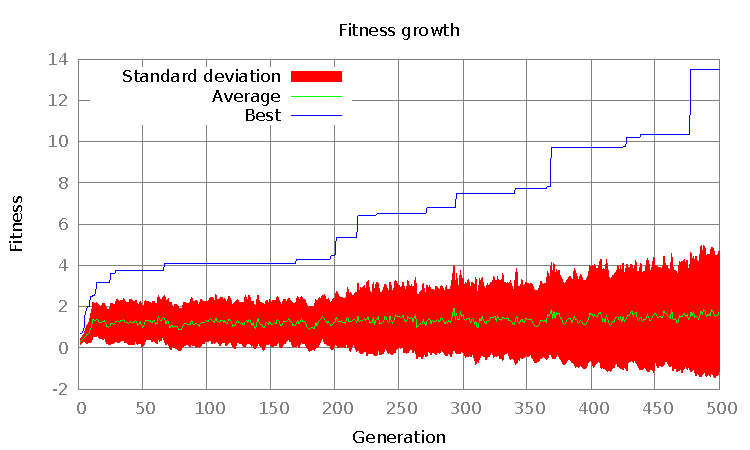
\includegraphics[width=\textwidth]{../output/wdm_izzy_1_fitness.pdf}
		\caption{Fitness progression for test case 3}
		\label{fig:fitness-test-case-3}
	\end{subfigure}%
	\begin{subfigure}[b]{0.5\textwidth}
		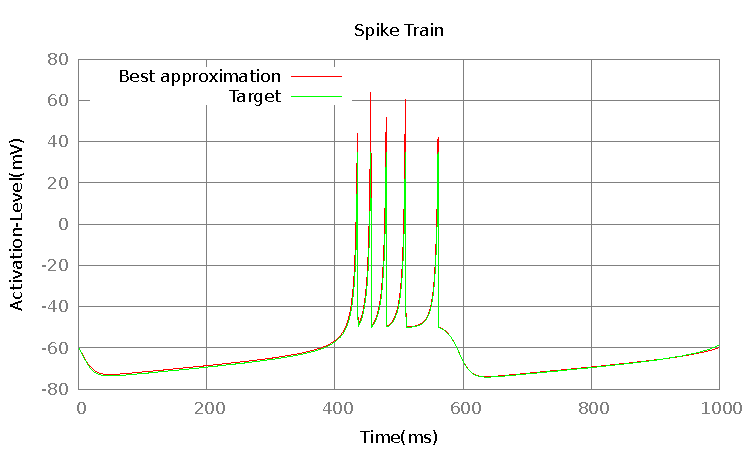
\includegraphics[width=\textwidth]{../output/wdm_izzy_1_spike.pdf}
		\caption{Spike train comparison for test case 3}
		\label{fig:spike-test-case-3}
	\end{subfigure}
	\caption{Test case 3 result}
\end{figure}

\subsection{Test Case 4}\label{sec:test-case-4}
In this test we are testing STDM with the test case
\textit{izzy-train2.dat}.
\subsubsection{EA Parameters}\label{sec:test-case-4-parameters}
\begin{lstlisting}[frame=single, language=bash, caption=Command-line to
replicate the results]
python src/main.py 500 5 50 --mutation=0.1 --cross_rate=0.9 full_generational
sigma --elite=3 stdm convert_neuron neuron_plot training\
data/izzy-train2.dat --bits_per_num=40
\end{lstlisting}
\begin{table}
	\begin{tabular}{c c}
		Variable & Value \\
		\hline
		Generations & 500 \\
		\hline
		Population size & 50 \\
		\hline
		Mutation rate & 0.1 \\
		\hline
		Crossover rate & 0.9 \\
		\hline
		Protocol & Full generational replacement \\
		\hline
		Mechanism & Sigma scaling \\
		\hline
		Elitism & 3 \\
		\hline
		Bits per number & 3 \\
	\end{tabular}
	\caption{EA parameters for test case 4}
\end{table}
\subsubsection{End Results}\label{sec:test-case-4-results}
In this we can again see that STDM is quite good a placing the spike about where
they should be, but it can't seem to place them perfect nor get the spacing
completely correct.

The fitness is again quite representative for my earlier concerns, but high
mutation combined with some elitism and crossover actually produce decent
results. We can see that the standard deviation increases along with the best
becoming better. This is again one which could probably run forever, but the
later increases was not large enough for me to warrant the longer run times.
\begin{table}
	\begin{tabular}{c c c c c}
		a & b & c & d & k \\
		\hline
		0.0229 & 0.2902 & -47.672 & 5.7082 & 0.0470
	\end{tabular}
	\caption{The neuron variables which gave the best solution for test case
	4}
\end{table}
\begin{figure}[h]
	\centering
	\begin{subfigure}[b]{0.5\textwidth}
		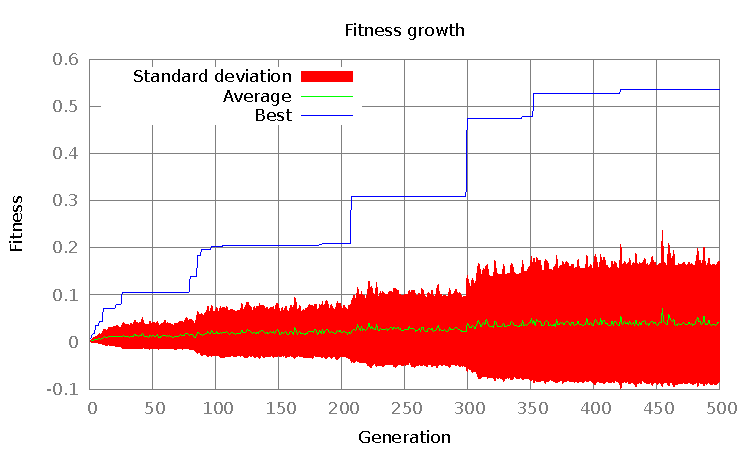
\includegraphics[width=\textwidth]{../output/stdm_izzy_2_fitness.pdf}
		\caption{Fitness progression for test case 4}
		\label{fig:fitness-test-case-4}
	\end{subfigure}%
	\begin{subfigure}[b]{0.5\textwidth}
		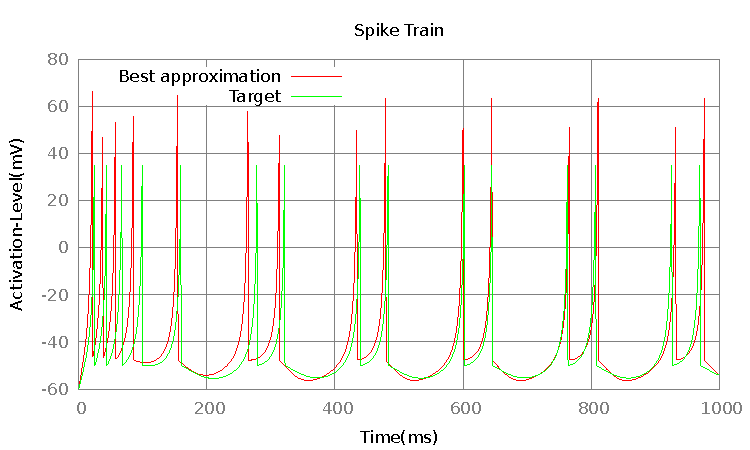
\includegraphics[width=\textwidth]{../output/stdm_izzy_2_spike.pdf}
		\caption{Spike train comparison for test case 4}
		\label{fig:spike-test-case-4}
	\end{subfigure}
	\caption{Test case 4 result}
\end{figure}

\subsection{Test Case 5}\label{sec:test-case-5}
In this test we are testing SIDM with the test case
\textit{izzy-train2.dat}.
\subsubsection{EA Parameters}\label{sec:test-case-5-parameters}
\begin{lstlisting}[frame=single, language=bash, caption=Command-line to
replicate the results]
python src/main.py 250 5 20 --mutation=0.1 --cross_rate=0.8 full_generational
tournament --k=5 --e=0.02 --elite=3 sidm convert_neuron neuron_plot training\
data/izzy-train2.dat --bits_per_num=40
\end{lstlisting}
\begin{table}
	\begin{tabular}{c c}
		Variable & Value \\
		\hline
		Generations & 250 \\
		\hline
		Population size & 20 \\
		\hline
		Mutation rate & 0.1 \\
		\hline
		Crossover rate & 0.8 \\
		\hline
		Protocol & Full generational replacement \\
		\hline
		Mechanism & Tournament, k=5, e=0.02 \\
		\hline
		Elitism & 3 \\
		\hline
		Bits per number & 40\\
	\end{tabular}
	\caption{EA parameters for test case 5}
\end{table}
\subsubsection{End Results}\label{sec:test-case-5-results}
This was one of those cases which probably ended up in a local maximum, since
changing any variable slightly would plummet the fitness far down. I chose to
include it because it was so good and in many cases no other case, so far, have
done as good with SIDM.

This case was again quite similar to the others in regard to fitness, it starts
out low and then increases. Again this is a test case which could have ran
longer, but trying to double the number of generations only gave an increase of
about 0.02 which I felt was not good enough.
\begin{table}
	\begin{tabular}{c c c c c}
		a & b & c & d & k \\
		\hline
		0.0313 & 0.1220 & -43.496 & 7.9364 & 0.0502
	\end{tabular}
	\caption{The neuron variables which gave the best solution for test case
	5}
\end{table}
\begin{figure}[h]
	\centering
	\begin{subfigure}[b]{0.5\textwidth}
		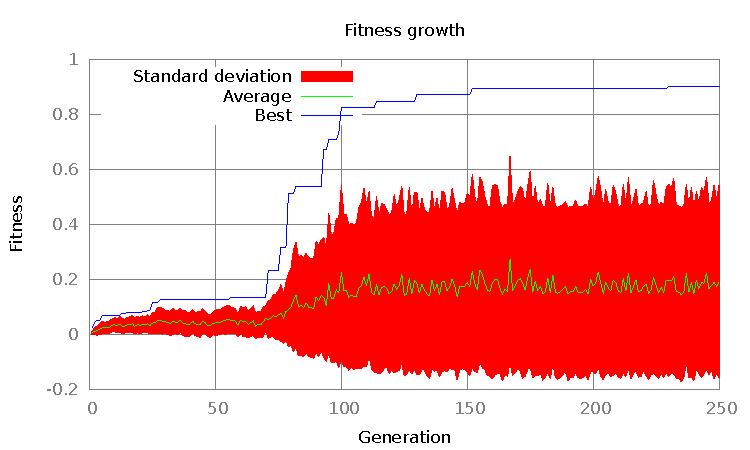
\includegraphics[width=\textwidth]{../output/sidm_izzy_2_fitness.pdf}
		\caption{Fitness progression for test case 5}
		\label{fig:fitness-test-case-5}
	\end{subfigure}%
	\begin{subfigure}[b]{0.5\textwidth}
		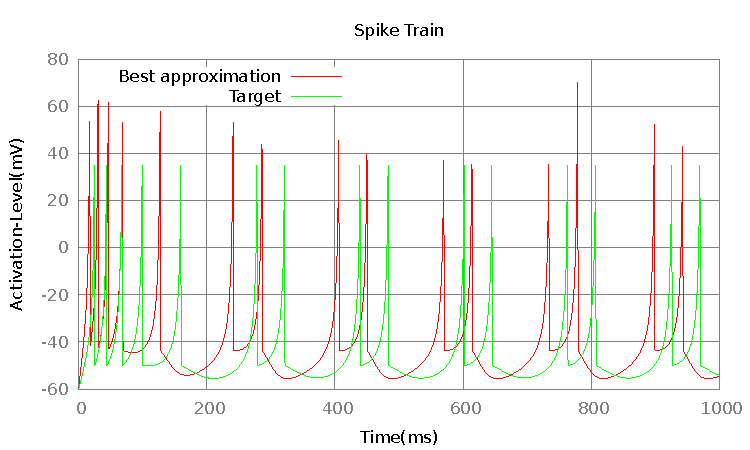
\includegraphics[width=\textwidth]{../output/sidm_izzy_2_spike.pdf}
		\caption{Spike train comparison for test case 5}
		\label{fig:spike-test-case-5}
	\end{subfigure}
	\caption{Test case 5 result}
\end{figure}

\subsection{Test Case 6}\label{sec:test-case-6}
In this test we are testing WDM with the test case
\textit{izzy-train2.dat}.
\subsubsection{EA Parameters}\label{sec:test-case-6-parameters}
\begin{lstlisting}[frame=single, language=bash, caption=Command-line to
replicate the results]
python src/main.py 400 5 50 --mutation=0.05 --cross_rate=0.9 full_generational
sigma --elite=3 wdm convert_neuron neuron_plot training\
data/izzy-train2.dat --bits_per_num=40
\end{lstlisting}
\begin{table}
	\begin{tabular}{c c}
		Variable & Value \\
		\hline
		Generations & 400 \\
		\hline
		Population size & 50 \\
		\hline
		Mutation rate & 0.05 \\
		\hline
		Crossover rate & 0.9 \\
		\hline
		Protocol & Full generational replacement \\
		\hline
		Mechanism & Sigma \\
		\hline
		Elitism & 3 \\
		\hline
		Bits per number & 40 \\
	\end{tabular}
	\caption{EA parameters for test case 6}
\end{table}
\subsubsection{End Results}\label{sec:test-case-6-results}
This test case seemed quite hard for WDM. No good results no matter the settings
tried which is very strange. The choice of going with Sigma scaling for this was
quite random as I tried several times with both this and Tournament selection
which came very close to each other and in the end I went with Sigma.

The fitness plot for this is also very strange, which again does not help
explain the results.
\begin{table}
	\begin{tabular}{c c c c c}
		a & b & c & d & k \\
		\hline
		0.0118 & 0.0538 & -55.717 & 8.2982 & 0.0569
	\end{tabular}
	\caption{The neuron variables which gave the best solution for test case
	6}
\end{table}
\begin{figure}[h]
	\centering
	\begin{subfigure}[b]{0.5\textwidth}
		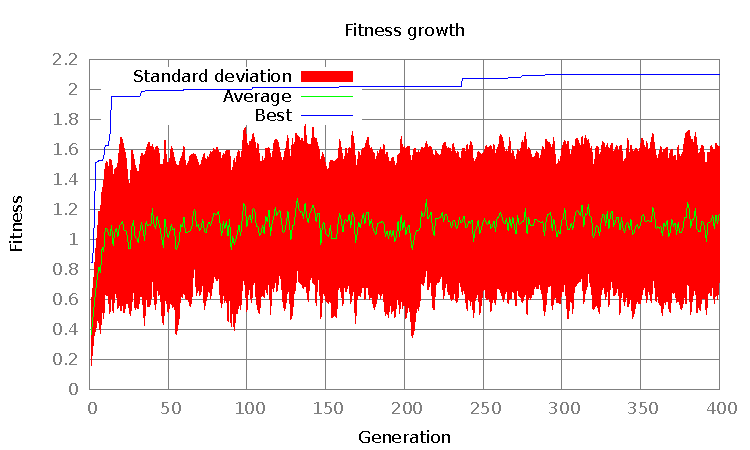
\includegraphics[width=\textwidth]{../output/wdm_izzy_2_fitness.pdf}
		\caption{Fitness progression for test case 6}
		\label{fig:fitness-test-case-6}
	\end{subfigure}%
	\begin{subfigure}[b]{0.5\textwidth}
		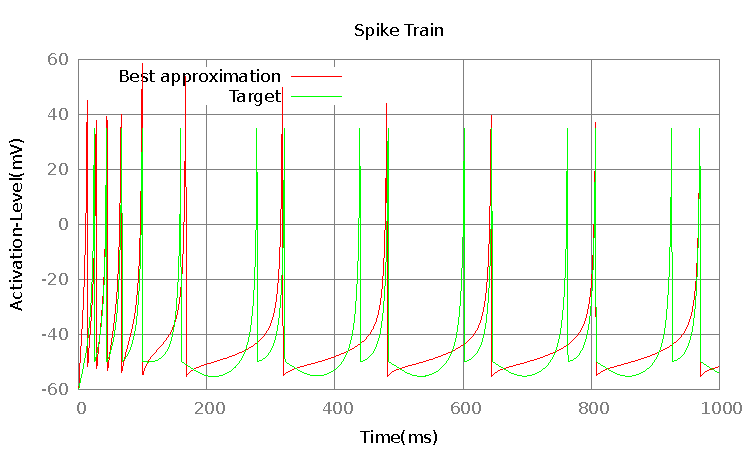
\includegraphics[width=\textwidth]{../output/wdm_izzy_2_spike.pdf}
		\caption{Spike train comparison for test case 6}
		\label{fig:spike-test-case-6}
	\end{subfigure}
	\caption{Test case 6 result}
\end{figure}

\subsection{Test Case 7}\label{sec:test-case-7}
In this test we are testing STDM with the test case
\textit{izzy-train3.dat}.
\subsubsection{EA Parameters}\label{sec:test-case-7-parameters}
\begin{table}
	\begin{tabular}{c c}
		Variable & Value \\
		\hline
		Generations & X \\
		\hline
		Population size & X \\
		\hline
		Mutation rate & X \\
		\hline
		Crossover rate & X \\
		\hline
		Protocol & X \\
		\hline
		Mechanism & X \\
		\hline
		Elitism & X \\
		\hline
		Bits per number & \\
	\end{tabular}
	\caption{EA parameters for test case 7}
\end{table}
\subsubsection{End Results}\label{sec:test-case-7-results}
\begin{table}
	\begin{tabular}{c c c c c}
		a & b & c & d & k \\
	\end{tabular}
\end{table}

\subsection{Test Case 8}\label{sec:test-case-8}
In this test we are testing SIDM with the test case
\textit{izzy-train3.dat}.
\subsubsection{EA Parameters}\label{sec:test-case-8-parameters}
\begin{table}
	\begin{tabular}{c c}
		Variable & Value \\
		\hline
		Generations & X \\
		\hline
		Population size & X \\
		\hline
		Mutation rate & X \\
		\hline
		Crossover rate & X \\
		\hline
		Protocol & X \\
		\hline
		Mechanism & X \\
		\hline
		Elitism & X \\
		\hline
		Bits per number & \\
	\end{tabular}
	\caption{EA parameters for test case 8}
\end{table}
\subsubsection{End Results}\label{sec:test-case-8-results}
\begin{table}
	\begin{tabular}{c c c c c}
		a & b & c & d & k \\
	\end{tabular}
\end{table}

\subsection{Test Case 9}\label{sec:test-case-9}
In this test we are testing WDM with the test case
\textit{izzy-train3.dat}.
\subsubsection{EA Parameters}\label{sec:test-case-9-parameters}
\begin{table}
	\begin{tabular}{c c}
		Variable & Value \\
		\hline
		Generations & X \\
		\hline
		Population size & X \\
		\hline
		Mutation rate & X \\
		\hline
		Crossover rate & X \\
		\hline
		Protocol & X \\
		\hline
		Mechanism & X \\
		\hline
		Elitism & X \\
		\hline
		Bits per number & \\
	\end{tabular}
	\caption{EA parameters for test case 9}
\end{table}
\subsubsection{End Results}\label{sec:test-case-9-results}
\begin{table}
	\begin{tabular}{c c c c c}
		a & b & c & d & k \\
	\end{tabular}
\end{table}

\subsection{Test Case 10}\label{sec:test-case-10}
In this test we are testing STDM with the test case
\textit{izzy-train4.dat}.
\subsubsection{EA Parameters}\label{sec:test-case-10-parameters}
\begin{table}
	\begin{tabular}{c c}
		Variable & Value \\
		\hline
		Generations & X \\
		\hline
		Population size & X \\
		\hline
		Mutation rate & X \\
		\hline
		Crossover rate & X \\
		\hline
		Protocol & X \\
		\hline
		Mechanism & X \\
		\hline
		Elitism & X \\
		\hline
		Bits per number & \\
	\end{tabular}
	\caption{EA parameters for test case 10}
\end{table}
\subsubsection{End Results}\label{sec:test-case-10-results}
\begin{table}
	\begin{tabular}{c c c c c}
		a & b & c & d & k \\
	\end{tabular}
\end{table}

\subsection{Test Case 11}\label{sec:test-case-11}
In this test we are testing SIDM with the test case
\textit{izzy-train4.dat}.
\subsubsection{EA Parameters}\label{sec:test-case-11-parameters}
\begin{table}
	\begin{tabular}{c c}
		Variable & Value \\
		\hline
		Generations & X \\
		\hline
		Population size & X \\
		\hline
		Mutation rate & X \\
		\hline
		Crossover rate & X \\
		\hline
		Protocol & X \\
		\hline
		Mechanism & X \\
		\hline
		Elitism & X \\
		\hline
		Bits per number & \\
	\end{tabular}
	\caption{EA parameters for test case 11}
\end{table}
\subsubsection{End Results}\label{sec:test-case-11-results}
\begin{table}
	\begin{tabular}{c c c c c}
		a & b & c & d & k \\
	\end{tabular}
\end{table}

\subsection{Test Case 12}\label{sec:test-case-12}
In this test we are testing WDM with the test case
\textit{izzy-train4.dat}.
\subsubsection{EA Parameters}\label{sec:test-case-12-parameters}
\begin{table}
	\begin{tabular}{c c}
		Variable & Value \\
		\hline
		Generations & X \\
		\hline
		Population size & X \\
		\hline
		Mutation rate & X \\
		\hline
		Crossover rate & X \\
		\hline
		Protocol & X \\
		\hline
		Mechanism & X \\
		\hline
		Elitism & X \\
		\hline
		Bits per number & \\
	\end{tabular}
	\caption{EA parameters for test case 12}
\end{table}
\subsubsection{End Results}\label{sec:test-case-12-results}
\begin{table}
	\begin{tabular}{c c c c c}
		a & b & c & d & k \\
	\end{tabular}
\end{table}
